% 鈍角の例：θ = 3π/4（135°）の点 P(-√2/2, √2/2)。x 軸の負の側と 45° をなす直角三角形で値を読む
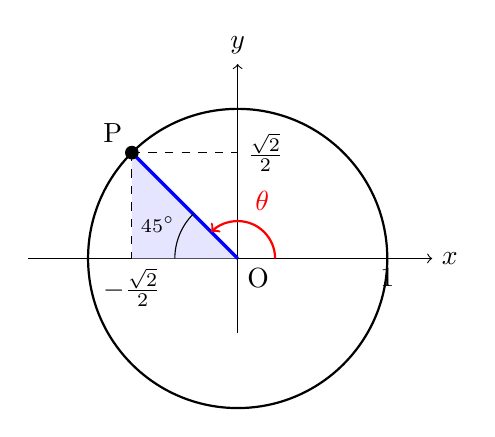
\begin{tikzpicture}[scale=1.9]
  \draw[->] (-1.4,0) -- (1.3,0) node[right] {$x$};
  \draw[->] (0,-0.5) -- (0,1.3) node[above] {$y$};
  \draw[thick] (0,0) circle (1);
  \coordinate (P) at (135:1);
  % 直角三角形（x 軸の負の側と 45°）
  \fill[blue!10] (0,0) -- (P) -- (P |- 0,0) -- cycle;
  \draw[very thick,blue] (0,0) -- (P);
  \draw[dashed] (P) -- (P |- 0,0) node[below] {$-\frac{\sqrt{2}}{2}$};
  \draw[dashed] (P) -- (0,0 |- P) node[right] {$\frac{\sqrt{2}}{2}$};
  % 角 θ = 135°（x 軸の正の向きから測る）
  \draw[->,red,thick] (0.25,0) arc (0:135:0.25);
  \node[red] at (67:0.42) {$\theta$};
  % 三角形の中の 45°
  \draw (-0.42,0) arc (180:135:0.42);
  \node[font=\scriptsize] at (157:0.58) {$45^\circ$};
  \fill (P) circle (1.3pt) node[above left] {$\mathrm{P}$};
  \node[below right] at (0,0) {$\mathrm{O}$};
  \node[below] at (1,0) {$1$};
\end{tikzpicture}
